\chapter{Grafikformate im Web}
\begin{table}[ht]
\begin{tabularx}{\linewidth}{>{\parskip1ex}X@{\kern4\tabcolsep}>{\parskip1ex}X}

\hfil\bfseries Rastergrafiken
&
\hfil\bfseries Vektorgrafiken
\\\cmidrule(r{3\tabcolsep}){1-1}\cmidrule(l{-\tabcolsep}){2-2}

%% PROS, seperated by empty line or \par
Aufteilung der Darstellungsfläche in meist gleichgroße und quadratische Teilflächen.\par
Zuweisung (Attributierung) von Farbwerten, Helligkeitswerten, Transparenzwerten zu den einzelnen Teilflächen.\par
\textcolor{green}{\large \textbf{$+$}} einfache Darstellung auf herkömmlichen rasterbasierten Ausgabegeräten (LCD, Laser, Tintenstrahldrucker)\par
\textcolor{green}{\large \textbf{$+$}} einfache Übernahme von natürlichen Darstellungen möglich\par
\textcolor{red}{\large{\textbf{$-$}}} Skalierbarkeit schlecht: Vergrößerung des Rasters

&

%% CONS, seperated by empty line or \par
Etablieren eines Koordinatensystems auf der Darstellungsfläche\par
Darstellung von geometrischen Grundformen.\par
Attributierung der Grundformen mit Position, Größe, Farbe, Helligkeit, Transparenz, Muster, Strichdaten, ... (letztere optional)\par
\textcolor{green}{\large \textbf{$+$}} nahezu unbegrenzte Skalierbarkeit\par
\textcolor{green}{\large{\textbf{$+$}}} auch vektorbasierte Ausgabegeräte verfügbar: Plotter, vektorbasierte CRT-Bildschirme\par
\textcolor{red}{\large{\textbf{$-$}}} Rendering ist recht aufwändig

\end{tabularx}
\end{table}

\section{Rasterbasierte Grafikformate}
Zuweisung von Farbe $\rightarrow$ Farbmodell: RGB (Rot+Grün+Blau)\\
Helligkeit ergibt sich durch die Farbwerte: größere Werte $\rightarrow$ mehr Helligkeit.\\
Üblicherweise wird jedem Farbanteil ein 8bit-Wert zugewiesen $\Rightarrow$ ein Bildpunkt benötigt $3*8bit=3Byte$\\
Bsp: Digitalkamera mit 25Megapixel $\Rightarrow$ 75MByte Speichervolumen pro Bild, 16GByte Speicherkarte $\Rightarrow$ „nur“ 200 Bilder $\Rightarrow$ Kompression der Speicherdaten!!!\\

\subsection{GIF}
Graphics Interchange Format wurde in den 1980er Jahren erfunden und verwendet das RGB-Farbmodell. Das Format ist für computergenerierte schematische Darstellung mit großen einfarbigen Flächen gut geeignet.
\paragraph{Manko}zu Beginn wird eine Farbtabelle mit maximal 256 Farben definiert und fortan jede Teilfläche nur noch mit einem 8bit Wert als Index auf diese Tabelle kodiert
\begin{itemize}
\item[$\Rightarrow$]Beschreibung der gleichzeitig verwendeten Farbenzahl auf 256 Farben (aus insgesamt $\approx$ 16Mio möglichen Farben)
\item[$\Rightarrow$]Reduktion der Datenmenge durch Verlust an Information (welcher klar sichtbar ist). Anschließende Kompression der Folge von Indexwerten: modifizierte Lauflängenkodierung (Wert und Anzahl)
\item[$\Rightarrow$]funktioniert bei häufig aufeinanderfolgenden Werten
\item[$\Rightarrow$]verlust\underline{freies} Kompressionsverfahren bei GIF!!!
\item[$\Rightarrow$]aber Voraussetzung für das Funktionieren des Kompressionsverfahrens ist die vorherige Reduktion auf 256 Farbwerte
\item[$\Rightarrow$]Wahrscheinlichkeit gleicher aufeinanderfolgender Werte damit recht hoch!
\end{itemize}
\paragraph{Transparenz} eine Farbe kann als transparent markiert werden, jedoch ist keine Teiltransparenz möglich.
\paragraph{Animated GIF}erlaubt kurze Sequenzen von Bildern, welche unmittelbar nacheinander dargestellt werden $\Rightarrow$ „Filmeffekt“

\subsection{JPEG}
Joint Photographic Expert Group verwendet das RGB-Farbmodell oder (alternativ) CMYK (für Druck)
\begin{itemize}
\item[$\Rightarrow$]keine Transparenz möglich
\item[$\Rightarrow$]keine Reduktion der Farbanzahl, also 16Mio. (bei RGB) bzw. 4Mrd. (bei CMYK) Farben gleichzeitig (theoretisch) möglich
\end{itemize}
\newpage
\subsubsection{DCT: Discrete Cosine Transform}
\begin{itemize}
\item[a)] Mittelwert über gesamtes (zunächst 8x8 Pixel) Areal
\item[b)] Halbierung des (8x8 Pixel-) Blockes in x- und y-Richtung auf vier (4x4 Pixel-) Blöcke
\item[c)] Berechnung der Mittelwerte dieser kleineren Blöcke
\item[d)] Abspeichern als Differenzen der kleinen Blöcke zum großen Block
\item[e)] weiter bis 1x1 Pixel-Block erreicht
\end{itemize}
DCT sorgt für denselben Informationsgehalt bei gleicher Datenmenge (keine Kompression!)\\
„Qualitätseinstellung“ durch Zusammenfassen von Koeffizienten mit ähnlichen Werten auf den gleichen Wert $\Rightarrow$ Informationsverlust, hilft der Effizienz des nachfolgenden Huffman

\paragraph{Huffman-Codierung: verlustfrei}abhängig von der Häufigkeit ihres Vorkommens werden die zu kodierenden Werte mit kürzeren oder längeren Codewerten dargestellt $\Rightarrow$ variabel lange Codeworte für die Werte!\\
Prinzip: Binärbaum\\
Beispiel:
\begin{table}[h]
\begin{tabular}{rcl}
0 & $\Rightarrow$ & fertig \\
1  & $\Rightarrow$ & kommt noch was\\
„0“  & $\Rightarrow$ & für häufigsten Wert\\
„10“  & $\Rightarrow$ & für zweithäufigsten Wert\\
„110“ & $\Rightarrow$ & für dritthäufigsten Wert\\
bis zu „11... 10“ (255 Einsen) & $\Rightarrow$ & für seltensten Werte
\end{tabular}
\end{table}\\
$\Rightarrow$funktioniert ganz gut bei DCT-Koeffizienten („Abweichungswerten“), da die Abweichungen häufig kleine Werte darstellen $\Rightarrow$ kurze Codelänge für diese kleinen Werte\\
$\Rightarrow$verlustfreie Komprimierung!

\subsubsection{Nachfolgeformat: JPEG2000}
\begin{itemize}
\item[$\Rightarrow$] unterstützt RGBA (zusätzlicher Alpha-Kanal/Transparenz mit 8bit)
\item[$\Rightarrow$] nur mit Lizenzgebühren zu verwenden
\item[$\Rightarrow$] keine weite Verbreitung bislang
\end{itemize}

\newpage

\subsection{PNG}
Portable Network Graphics wurde in den 1990er Jahren als Ersatz für GIF entwickelt (wg. Patentproblematik)
\paragraph{2 Modi:} \begin{itemize} \item indizierte Farben wie bei GIF
\item unreduzierte RGBA-Farben\end{itemize}
$\Rightarrow$beliebige (auch Teil-)Transparenz möglich. In jedem Fall verlustfreie Kompression nachgeschaltet.\\
$\Rightarrow$für photorealistische Darstellungen of deutlich größeres Dateivolumen als bei JPEG! Dafür evtl. JNG $\rightarrow$ keine große Verbreitung.

\section{Vektorgrafikformate}
\subsection{SVG}
Das Scalable Vector Graphics Format gibt es seit deren Einführung im Jahre 1998. Dabei gab es zwei unterschiedliche Vorschläge für das Vektorgrafikformat:
\begin{itemize}
\item VML (Vector Markup Language) von Microsoft
\item PGML (Precision Graphics Markup Language) von Adobe, IBM, NS/Netscape, Sun
\end{itemize}

\subsubsection{Historie}
10/1998: Entwurf für Anforderungen an VektorGrafikformat SVG\\
09/2001: SVG 1.0 als W3C-Standard\\
01/2003: SVG 1.1 mit errata, modularization\\
04/2005: SVG 1.2 verschiedene Profile („tiny“, „full“, „basic“). Bis auf „tiny“ wieder zurückgegangen\\
derzeit Arbeit an SVG2 ...\\
\\
SVG ist XML-basiert und benutzt als übliche File-Extension „.svg“.\\
MIME-Type: image/svg+xml\\

\subsubsection{SVG Viewer}
\begin{tabularx}{\textwidth}{lX}
früher: & Adobe SVG Viewer\\
heute: & native Unterstützung in allen gängigen Browsern (Mozilla Firefox, Google Chrome, Apple Safari, Opera Browser, Microsoft Internet Explorer)
\end{tabularx}

\subsubsection{SVG Editor}
Texteditor\\
XML-Editor\\
Inkscape\\
\begin{lstlisting}[caption={Grundgerüst einer SVG-Datei}, label={lst:Grundger:SVG}, language={XML}]
  <?xml version="1.0" [encoding="UTF-8"]?>
  <!DOCTYPE 
      svg <!--root-Tag-->
      PUBLIC <!--entspr. standardisierte Sprache-->
      "-//W3C//DTD SVG 1.1//EN" <!--Public Identifier-->
      "http://www.w3.org/Graphics/SVG/1.1/DTD/svg11.dtd" <!--System-Identifier-->
  >
  <svg
      xmlns="http://www.w3.org/2000/svg"
      [xmlns:xlink="http://www.w3.org/1999/xlink"]
      width="breite" height="hoehe" [viewBox="xlo ylo kbreite khoehe"]
  >
    <title>Name der Grafik</title>
    <desc>Beschreibung als Text</desc>
    <defs>
      <!--Platz fuer CSS-Definition, Javascript-Code, Definitionen von graph Objekten, welche zunaechst nicht angezeigt werden-->
    </defs>
    <!--eigentlicher Inhalt in Form von graph. Grundformen und unter Benutzung von komplexen (auch ind <defs> definierten) graph. Objekten-->
\end{lstlisting}
breite, hoehe: dimensionsbehaftete Angabe (z.b. 30mm, 500px) dimmensionslose Angabe äquivalent zu Pixel 3000\^=3000px\\
$\Rightarrow$durch breite und hoehe wird auch das Koordinatensystem aufgespannt...
\begin{figure}[h]
  \centering
  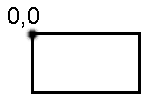
\includegraphics[scale=0.3]{svg-width-height.png}
  \caption{implizites Koordinatensystem in SVG durch Breiten- bzw. Höhenangaben}
\end{figure}\\
...wenn nicht auch das Attribut viewBox verwendet wird: viewBox=„xlo ylo kbreite khoehe“

\subsubsection{Grafische Grundformen}
Tags mit Attributen für Koordinaten und/oder Größe
\begin{lstlisting}[caption={Syntax von grafischen Grundformen in SVG}, label={lst:Grundger:SVG}, language={SVG}]
  <line x1="..." y1="..." x2="..." y2="..." />
  <!--Linie von Punkt(x1,y1) zu Punkt(x2,y2)-->
  
  <circle cx="..." cy="..." r="..." />
  <!--Kreis mit Mittelpunkt(cx,cy) und Radius r-->
  
  <rect x="..." y="..." width="..." height="..." />
  <!--lotrechtes Rechteck mit Eckpunkt(x,y), Breite width und Hoehe height-->
  
  <ellipse cx="..." cy="..." rx="..." ry="..." />
  <!--lotrechte Ellipse mit Mittelpunkt(cx,cy) und horizontalen bzw. vertikalen Radius rx bzw. ry-->
  
  <polyline points="x1 y1 x2 y2 x3 y3 ..." />
  <!--Streckenzug, welcher die Punkte(x1,y1),(x2,y2),(x3,y3),... verbindet, deren Koordinaten als paarweise Werte in einem Attribut angegeben werden-->
  <!--Koordinaten werden durch Leerzeichen und/oder Komma getrennt. Sinnvoll ist es jeweils aufeinanderfolgende x- und y-Koordinate desselben Punktes durch Komma und die Koordinaten des naechsten Punktes davon durch Leerzeichen zu trennen-->
  
  <polygon points="..." />
  <!--geschlossener Streckenzug, bis der letzte Punkt wieder mit dem ersten verbunden wird-->
\end{lstlisting}
bislang fehlen uns „runde Kurven“ bzw. „Kurvenzug“\\
Voraussezung: Funktion stetig und Funktion stetig differenzierbar d.h. die erste Ableitung=Steigung muss ebenfalls stetig sein.\\
Lösung: abschnittsweise Definition über (perse) stetig differenzierbare Funktionen; an den Schnittstelllen muss jeweils die Steigung der linken gleich der Steigung der rechten Kurve sein.\\
$\Rightarrow$Kurveninterpolation\\
bei SVG: Kurveninterpolation mittels „Bezierkurven“\\

\subsubsection{Bezierkurven}
\paragraph{quadratische Bezierkurve}
geometrische Herleitung von quadratischen Bezierkurven:
quadr.Bez.-Kurve wird vollständig über drei Punkte definiert:
\begin{itemize}
\item Anfangspunkt (AP)
\item Stützpunkt (SP)
\item Endpunkt (EP)
\end{itemize}
\textbf{Eigenschaften:} Die Kurve beginnt im Anfangspunkt und endet im Endpunkt. Der Stützpunkt liegt im allgemeinen nicht auf der Kurve.\\
Kurve hat im AP die Steigung der Geraden AP-SP und im EP die Steigung der Geraden SP-EP.
\paragraph{kubische Bezierkurve}
AP-SP1-SP2-EP\\
beginnt in AP und endet in EP, Steigung in AP \^= Steigung AP-SP1, Steigung in EP \^= Steigung SP2-EP.\\
\paragraph{De-Casteljau-Algorithmus}
allgemeiner Tag zum Zeichnen von u.a. auch Bezier-Kurven:
\begin{lstlisting}[caption={Path-Tag}, label={lst:path-Tag}, language={SVG}]
  <path d="...." />
\end{lstlisting}
Das d- (wie „data“)-Attribut enthält eine Art „Zeichenbefehle“, mit denen das Ergebnis des path-Tags spezifiziert wird, sowie die entsprechenden (Punkt-)Koordinaten.\\
\\
\textbf{Zeichenbefehle:} 1Buchstaben, gefolgt von den zugehörigen Koordinaten\\
$\rightarrow$Großbuchstaben: absolute Koordinaten\\
$\rightarrow$Kleinbuchstaben: relative Koordinaten, d.h. relativ zur aktuellen (letzten) Position\\
$\Rightarrow$Wir bewegen uns während des Abarbeitens des path-Tags über die Darstellungsfläche.\\
$\Rightarrow$zu Beginn des path-Tags befinden wir uns um Ursprung (bei (0,0)).\\
„M“ („More“)$\Rightarrow$bewegt den Zeichenstift, ohne etwas zu zeichnen\\
\begin{lstlisting}[caption={Beispiel für "M" im Path-Tag}, label={lst:BSP:M-path-Tag}, language={SVG}]
  <path d="M10,50 m30,-20" />
\end{lstlisting}
Im Beispiel aus Listing\vref{lst:BSP:M-path-Tag} ändert sich die Position zu (40,30), ohne etwas zu zeichnen.\\
„L“ („Line“)$\Rightarrow$zeichnet eine Strecke vom aktuellen zum neuen Punkt
\begin{lstlisting}[caption={Beispiel für "L" im Path-Tag}, label={lst:BSP:L-path-Tag}, language={SVG}]
  <path d="M10,50 m30,-20 L70,20 m10,10 l-20,-50" />
\end{lstlisting}
Das Baispiellisting\vref{lst:BSP:L-path-Tag} zeichnet eine Strecke (40,30)-(70,20) und eine Strecke (80,30)-(60,-20)\\
\\
\begin{tabularx}{\textwidth}{lcX}
$M x1 y1$ & $\Rightarrow$ & $x_{a}=x1, y_{a}=y1$\\
$m dx dy$ & $\Rightarrow$ & $x_{a}=x_{a}+dx, y_{a}=y_{a}+dy$\\
$L x1 y1$ & $\Rightarrow$ & zeichnet Strecke von $(x_{a},y_{a})$ zu (x1,y1) und verändert $x_{a}=x1, y_{a}=y1$\\
$l dx dy$ & $\Rightarrow$ & zeichnet Strecke von $x_{a},y_{a}$ nach $(x_{a}+dx, y_{a}+dy)$ und verändert $x_{a}=x_{a}+dx,y_{a}=y_{a}+dy$\\
$H x1$ & $\Rightarrow$ & zeichnet horizontale Strecke von $(x_{a},y_{a}$ nach $(x1,y_{a})$ und verändert $x_{a}=x1,y_{a}=y_{a}$
h dx $\Rightarrow$Strecke von $(x_{a},y_{a})-(x_{a}+dx,y_{a})$ und $x_{a}=x_{a}+dx,y_{a}=y_{a}$\\
$V y1 \vee$ v dy & $\Rightarrow$ & zeichnet eine vertikale Strecke entsprechend\\
\end{tabularx}
\begin{lstlisting}[caption={Beispiel für "L" im Path-Tag}, label={lst:BSP:L-path-Tag}, language={SVG}]
  <polyline points="30,20 50,10 70,70" />
  <path d="M30,20 L50,10 L70,70" />
  <!--oder-->
  <path d="M30,20 l20,-10 l20,60" />
\end{lstlisting}
\begin{tabularx}{\textwidth}{llX}
Q sx,sy ex,ey & $\Rightarrow$ & quadratische B-K mit AP$(x_{a},y_{a})$, SP$(sx,sy)$, EP$(ex,ey)$\\
q sdx,sdy edx,edy & $\Rightarrow$ & quadratische B-K mit AP$(x_{a},y_{a})$, SP$(x_{a}+sdx,y_{a}+sdy)$, EP$(x_{a}+edx,y_{a}+edy)$\\
\multicolumn{3}{l}{Achtung:}„Während“ der Abarbeitung des einzelnen Befehls bleibt $(x_{a},y_{a})$ auf dem Anfangspunkt.\\
(s1x,s1y s2x,s2y ex,ey) & $\Rightarrow$ & kubische B-K mit AP$(x_{a},y_{a})$, SP1$(s1x,s1y)$, SP2$(s2x,s2y)$, EP$(ex,ey)$\\
c s1dx,s1dy s2dx,s2dy ex,ey & $\Rightarrow$ & kubische Bezier-Kurve entsprechend mit relativen Koordinaten\\
T ex,ey & $\Rightarrow$ & quadratische Bezier-Kurve mit von der vorherigen B-K an AP gespiegelten SP\\
S s2x,s2y ex,ey & $\Rightarrow$ & kubische B-K mit von der vorigen kubischen B-K an AP zu SP1 gespiegelten SP2\\
\end{tabularx}
\\
$\Rightarrow$sinnvoll (nur) bei voriger quadr. bzw. kubischer Bezier-Kurve\\
falls nicht$\Rightarrow$SVG-Spezifikation gibt an, wie der zu spiegelnde Punkt zu bestimmen ist\\
\\
\begin{tabularx}{\textwidth}{lX}
A,a:„elliptical arc“ & $\Rightarrow$zeichnet Ausschnitt aus Ellipsen\\
 & $\Rightarrow$relativ schwer zu verwenden (Parameter selbst nachlesen!)\\
Z,z: & schließt den aktuellen Streckenzug mit einer Strecke zum entsprechenden ersten Punkt (nach dem letzten M-Befehl)
\end{tabularx}
\begin{lstlisting}[caption={Beispiel zwei Dreiecke mit nur einem Path-Tag}, label={lst:BSP:L-path-Tag}, language={SVG}]
  <path d="M10,10 L20,10 L15,20 Z M60,30 L70,40 L50,60 Z" />
  <!-- Z=zurueck zu Anfangspunkt -->
\end{lstlisting}

\subsubsection{Text}
\begin{lstlisting}[caption={Syntax des Text-Tag}, label={lst:text-Tag}, language={SVG}]
  <text x="x" y="y">Text der dargestellt wird</text>
\end{lstlisting}
$\Rightarrow$erstellt einen einzeiligen Text, beginnend an der Position (x,y)\\
$\Rightarrow$Zeichenumbrüche sind zunächst nicht möglich\\
aber: innerhalb <text> kann der Text mit <tspan> logisch unterteilt werden
\begin{lstlisting}[caption={Syntax des Text-Tag}, label={lst:Syntax des tspan-Tag}, language={SVG}]
  <tspan[x="x" y="y"]>Text, welcher an einer Position (durch die optionalen Attribute x und y gegeben) beginnen kann</tspan>
  <tspan [dx="dx" dy="dy"]>Text,welcher an einer Position mit Versatz (dx,dy) zur letzten Position gesetzt wird<\tspan>
\end{lstlisting}
$\Rightarrow$mehrzeiliger Text mit etwas Aufwand und ungewohnt, aber machbar\\
\begin{lstlisting}[caption={Beispiel für ein tspan-Tag}, label={lst:text-Tag}, language={SVG}]
  <text x="0" y="0">
    <tspan>eins</tspan>
    <tspan x="0" dy="10">anderthalb</tspan>
    <tspan x="0" dy="10">zwei</tspan>
    <tspan x="0" dy="10">drei</tspan>
  </text>
\end{lstlisting}
Universalattribute:\\
style: für CSS-Deklarationen (wie bei HTML, allerdings größtenteils andere Properties)\\
\begin{lstlisting}[caption={Gruppierung von Inhalts-Tags bei SVG}, label={lst:text-Tag}, language={SVG}]
  <g><!-- beliebige andere Tags fuer grafische Grundelemente, Text, fuer weitere Gruppen -->
\end{lstlisting}

\subsubsection{CSS-Properties für SVG}
stroke: Strichfarbe $\Rightarrow$ z.b. „line \{stroke: red;\}“\\
stroke: \#ABCDEF;\\
stroke: \#AFE; \^= \#AAFFEE\\
stroke: rgb(0,200,0);\\
\\
opacity: 0.5; („Deckkraft“)\\
0: voll-transparent\\
1: voll-deckend/intransparent\\
\\
fill: Füllfarbe\\
\\
opacity bestimmt die Deckkraft gleichermaßen für Strich und Füllung, getrennt mögich über\\
stroke-opacity:1.0;\\
fill-opacity:0.2;\\
\\
stroke-width: Strichdicke\\
strocke-width:2px;\\
$\Rightarrow$Strichdicke von 2„Pixeln“=Einheiten im User Coordinate System
